\documentclass[../../Cours_M1.tex]{subfiles}

\newcommand{\nomTD}{TP3: Modulation et démodulation d'amplitude}
\renewcommand{\nomentete}{UE431 - \nomTD}
\renewcommand{\auteur}{Aymeric Arnould, Tom Colinot}

\title{\nomTD}
\author{\auteur}

\renewcommand{\thesection}{\Roman{section}}
\renewcommand{\thesubsection}{\arabic{subsection}}

\begin{document}

\maketitle

\begin{center}
\begin{Large}
A. Préparation
\end{Large}
\end{center}

\section{La modulation d'amplitude}

\subsection{Définitions}

\begin{itemize}
\item On s'intéresse à la transmission d'un signal informatif $s_{inf}(t)$ de spectre borné $[F_{min},F_{max}]$. Ici, on prend un signal sinusoïdal $s_{inf}(t) = S_m\cos(\Omega t)$. \\

Le signal porteur est $p(t)=S_p\cos(\omega_0 t)$, avec $\omega_0 >> \Omega$.\\

\item Les expressions des signaux modulés en amplitude sont alors :

\begin{multicols}{2}
- pour la modulation à double bande latérale à porteuse conservée (DBPC) :
\[s(t)=S_p[1+m\cos(\Omega t)]\cos(\omega_0 t)\]
- pour la modulation à double bande latérale à porteuse supprimée (DBPS) :
\[s(t)=S_p[m\cos(\Omega t)]\cos(\omega_0 t)\]
\end{multicols}
\end{itemize}

\subsection{Caractéristiques d'une onde modulée en amplitude}

\subsubsection{Analyse temporelle}

On peut tracer, à l'aide de Matlab, des signaux modulés. Ici $s_{inf}(t)$ est sinusoïdal, avec $S_m=0,8,\quad \Omega=2rad/s$, et $S_p=1,2,\quad \omega_0=100rad/s$.
\begin{figure}[h!]
\centering
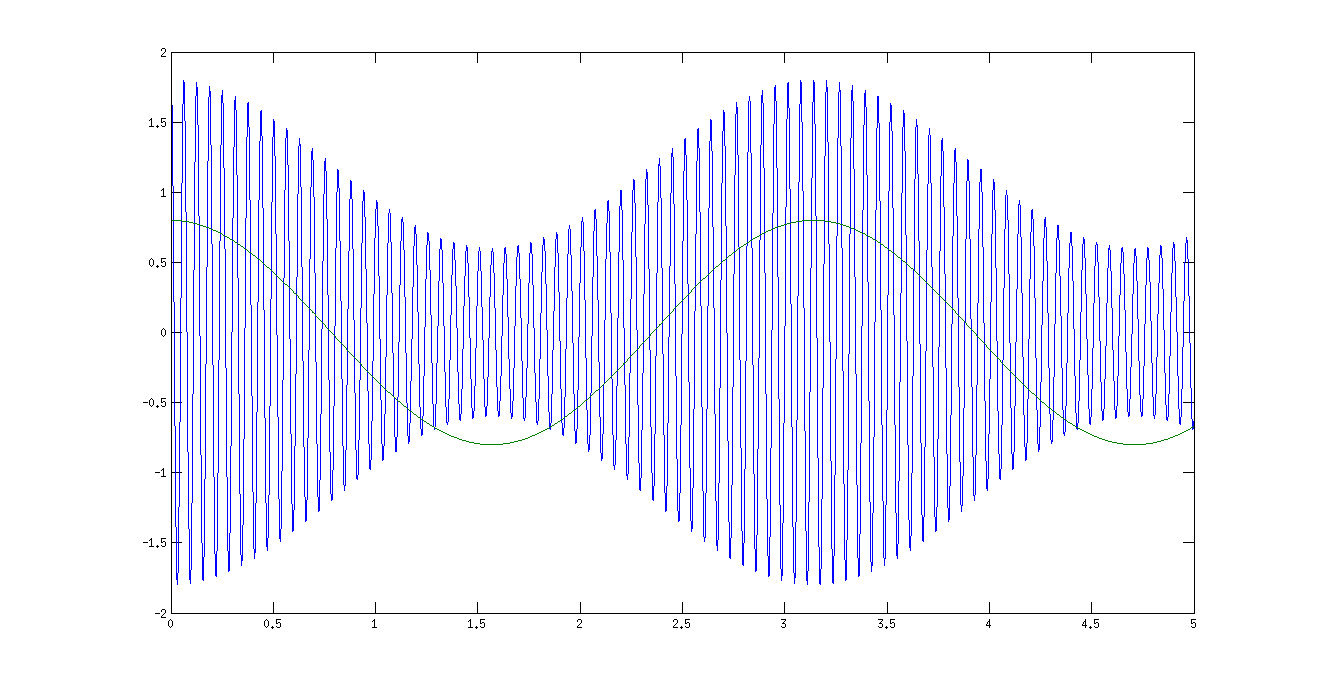
\includegraphics[scale=0.16]{DBPC05.png}
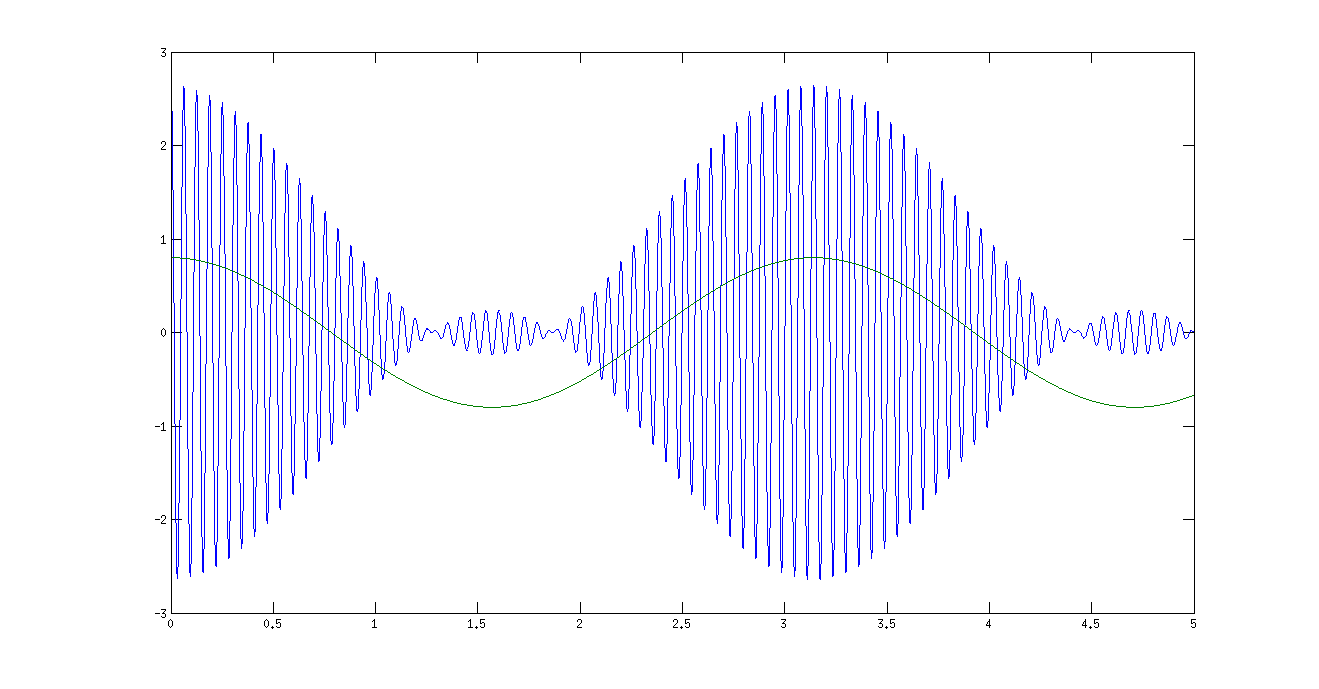
\includegraphics[scale=0.16]{DBPC12.png}
\caption{DBPC : Allures de $s(t)$ et $s_{inf}(t)$, pour m = 0,8 puis m = 1,2}
\end{figure}
\begin{figure}[h!]
\centering
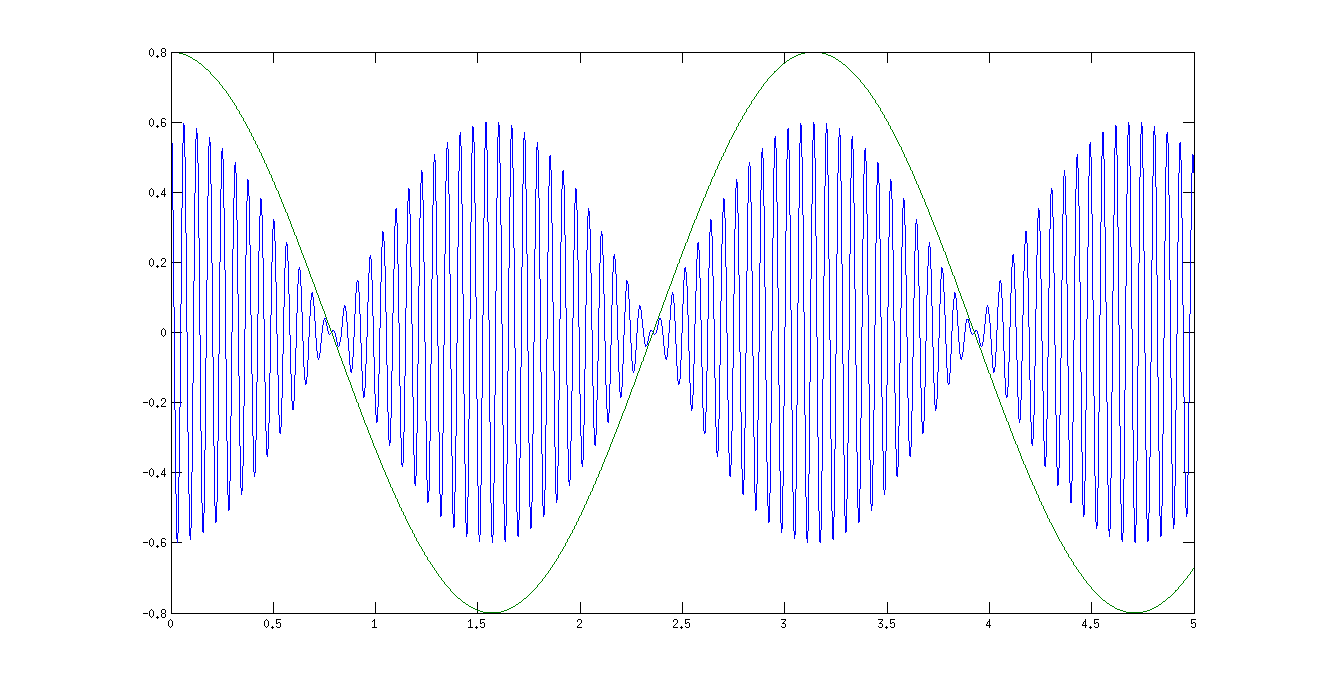
\includegraphics[scale=0.16]{DBPS.png}
\caption{DBPS : Allures de $s(t)$ et $s_{inf}(t)$}
\end{figure}

\subsubsection{Analyse spectrale}

Dans le cas d'un signal modulant sinusoïdal, on a
\begin{itemize}
\item en DBPC :
\[ s(t) = S_p[1+m\cos(\Omega t)]\cos(\omega_0(t)) = S_p\cos(\omega_0 t) + \frac{S_p m}{2}[\cos((\omega_0-\Omega)t)+\cos((\omega_0+\Omega)t)]\]
Le spectre de $s(t)$ est donc constitué de trois raies, deux raies d'amplitude $\frac{S_p m}{2}$ à $\omega_0-\Omega$ et $\omega_0+\Omega$, de part et d'autre d'une raie à $\omega_0$ d'amplitude $S_p$.

\begin{figure}[h!]
\centering
\begin{tikzpicture}
\draw [>=latex,->] (0,0) -- (6,0) node[right]{$\omega$} ;
\draw [>=latex,->] (0,0) -- (0,3) node[left]{$Amplitude$};
\draw (4,0)node[below]{$\omega_0$} -- (4,2);
\draw (3,0)node[below]{$\omega_0-\Omega$} -- (3,1);
\draw (5,0)node[below]{$\omega_0+\Omega$} -- (5,1);
\draw [dotted] (0,2) node[left]{$S_p$} -- (6,2);
\draw [dotted] (0,1) node[left]{$\frac{S_p m}{2}$} -- (6,1);

\end{tikzpicture}
\caption{Spectre de $x(t)$ dans le cas DBPC}
\end{figure}

\item en DBPS :
\[ s(t) = S_p[m\cos(\Omega t)]\cos(\omega_0(t)) = \frac{S_p m}{2}[\cos((\omega_0-\Omega)t)+\cos((\omega_0+\Omega)t)]\]
Le spectre de $s(t)$ est donc constitué de deux raies d'amplitude $\frac{S_p m}{2}$ à $\omega_0-\Omega$ et $\omega_0+\Omega$.

\begin{figure}[h!]
\centering
\begin{tikzpicture}
\draw [>=latex,->] (0,0) -- (6,0) node[right]{$\omega$} ;
\draw [>=latex,->] (0,0) -- (0,3) node[left]{$Amplitude$};
\draw (3,0)node[below]{$\omega_0-\Omega$} -- (3,1);
\draw (5,0)node[below]{$\omega_0+\Omega$} -- (5,1);
\draw [dotted] (0,1) node[left]{$\frac{S_p m}{2}$} -- (6,1);

\end{tikzpicture}
\caption{Spectre de $x(t)$ dans le cas DBPS}
\end{figure}

\end{itemize}

Avec un analyseur de spectres (qui trace le spectre du signal temporel), on peut déterminer le type de modulation en comptant le nombre de raies (DBPC s'il y a 3 raies, DBPS s'il y en a 2). La visualisation du spectre donne également l'encombrement spectral du signal modulé (ici, $\frac{2\Omega}{2\pi}$.)

\subsubsection{Mesure du taux de modulation m}

\begin{itemize}
\item \emph{Analyse spectrale :} d'après l'étude précédente dans le cas DBPC, si on pose $A_{\omega_0}$ (resp. $A_{\omega_0-\Omega}$) l'amplitude de la composante à $\omega_0$ (resp. $\omega_0-\Omega$) de $s(t)$, alors \[m=\frac{2A_{\omega_0-\Omega}}{A_{\omega_0}}\]

\item \emph{Visualisation de l'onde modulée en amplitude :} dans le cas DBPC, \[s(t) = S_p[1+m\cos(\Omega t)]\cos(\omega_0 t)\]
En notant $Max$ le maximum de l'enveloppe du signal, $min$ le minimum, on a
\[m= 2\frac{Max-min}{Max+min}\]

\item \emph{Méthode du trapèze :} dans le cas DBPC, en traçant $s(t)$ en fonction de $s_{inf}(t)$, avec l'oscilloscope en mode X-Y :
\begin{figure}[h!]
\centering
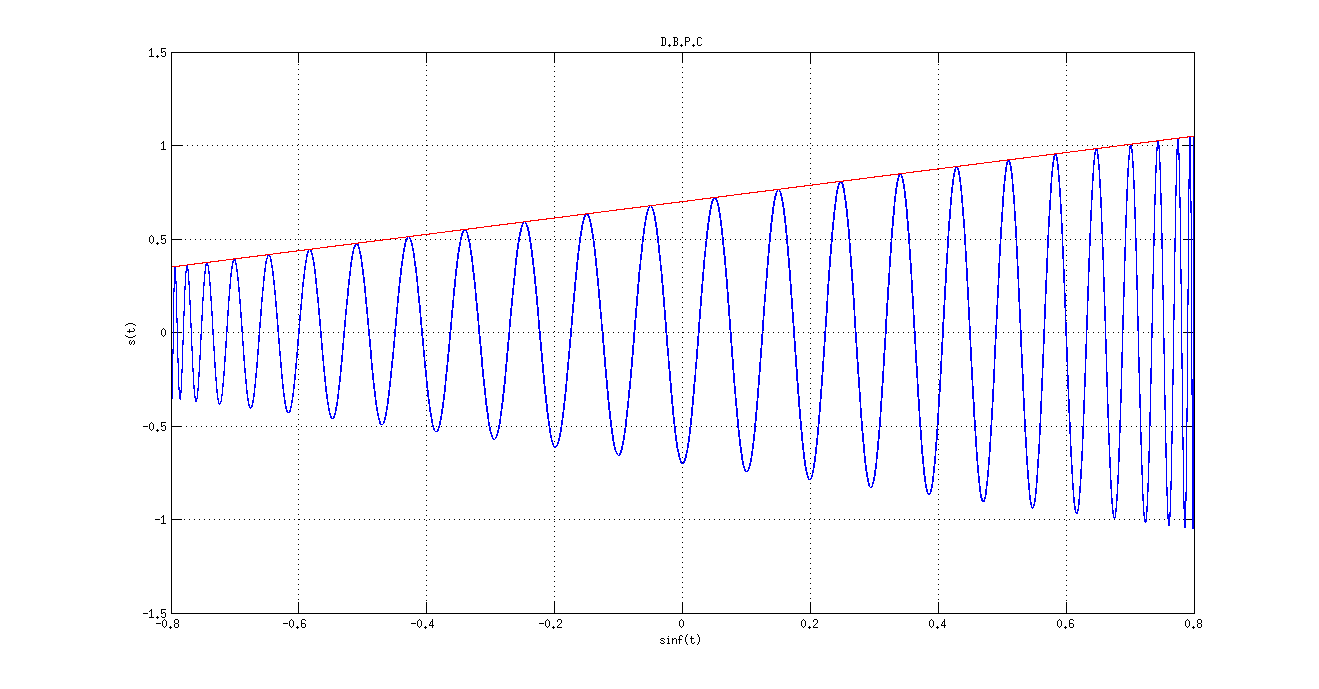
\includegraphics[scale=0.4]{DBPCXY.png}
\caption{Tracé de $s(t)$ en fonction de $s_{inf}(t)$, DBPC}
\end{figure}
En effet, on a : $s(t) = S_p(1+ks_{inf}(t))\cos(\omega_0 t)$

L'enveloppe tracée en rouge est donc la droite $y(t)=S_p(1+ks_{inf}(t))$. Ainsi, $S_p$ est l'ordonnée à l'origine de cette droite, et $kS_p$ est sa pente. 

De plus, comme $s_{inf}(t)=S_m\cos(\Omega t)$, $s_{inf}$ varie entre $-S_m$ et $S_m$ qui définissent l'axe des abscisses sur lequel le tracé a été effectué.\\

Dans le cas DBPS, le même tracé donne :
\begin{figure}[h!]
\centering
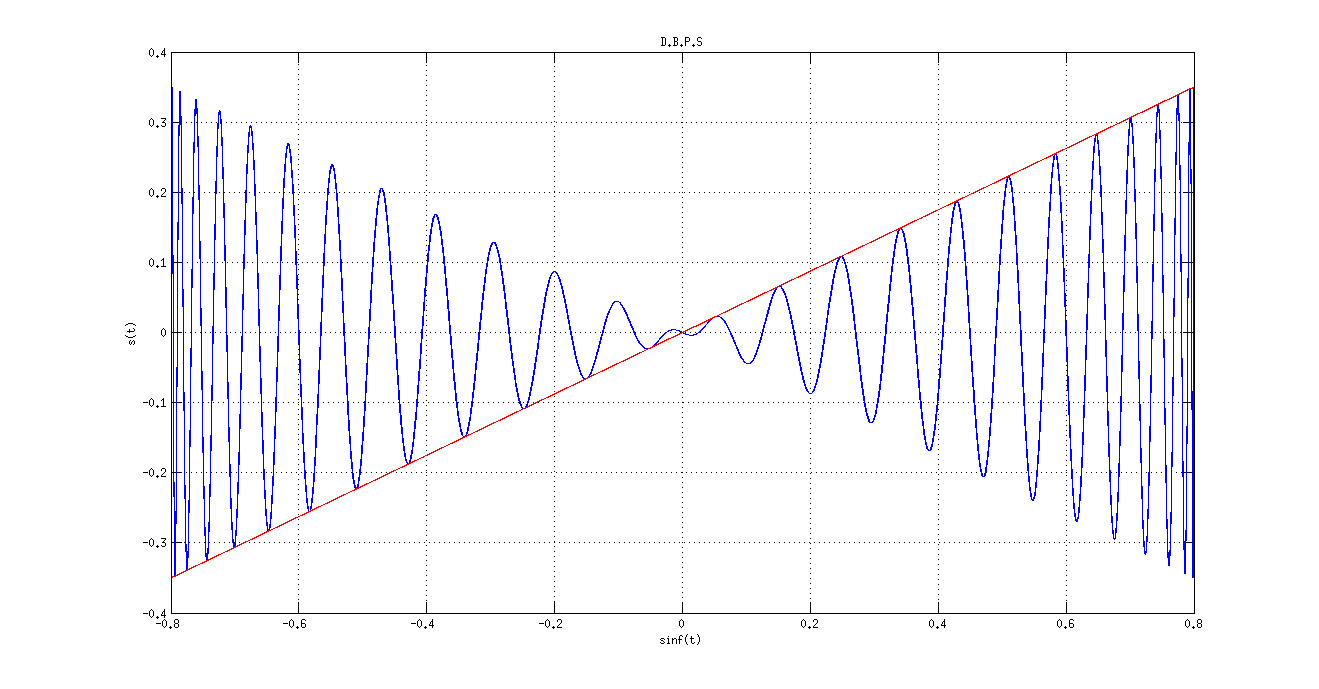
\includegraphics[scale=0.4]{DBPSXY.png}
\caption{Tracé de $s(t)$ en fonction de $s_{inf}(t)$, DBPS}
\end{figure}

On sait que \[s(t) = S_pks_{inf}(t)\cos(\omega_0 t)\]
L'enveloppe tracée en rouge est donc une droite de pente $S_pk$ passant par l'origine. Comme précédemment, on a aussi la valeur de $S_m$ par lecture sur l'axe des abscisses. On peut donc en déduire la valeur de $m=kS_m$.\\

La méthode précédente fournissait les valeurs de $m$ et $S_p$. Ici, on a aussi accès à $S_m$ (ou $k$).
\end{itemize}

\section{Techniques de démodulation d'amplitude}

\subsection{Démodulation par détection d'enveloppe et filtrage}

\begin{itemize}
\item \emph{Principe :} lorsque $s(t)$ est positive et augmente, la capacité se charge et $r(t) = s(t)$.

Lorsque $s(t)$ est maximale puis décroît, alors $s(t) < r(t)$ et $D_1$ se bloque : $C_1$ se décharge dans $R_1$ et $r(t)$ décroît selon une loi exponentielle.

Il faut alors bien choisir $R_1$ et $C_1$ pour que la décharge ne soit pas trop rapide, afin que $r(t)$ ne varie pas trop entre deux pics maxima consécutifs de $s(t)$. 
\item Lors de la décharge de $C_1$ dans $R_1$ (aucun courant ne traverse la diode) :
\[ r(t) = -R_1C_1\frac{dr(t)}{dt} \]
\item On en déduit donc
\[ r(t) = r_0e^{-\frac{t-t_1}{R_1C_1}} \] où $r_0$ est la valeur en début de décharge, c'est-à-dire la valeur de $s(t)$ en $t=t_1$. Cette valeur est le maximum du signal $s(t)$, soit $S_p(1+m\cos(\Omega t_1))$. \\
La pente de la droite de décharge du condensateur à l'instant $t_1$ est donc \[\frac{dr(t)}{dt_1}|_{t=t_1}= -\frac{S_p}{R_1C_1}(1+m\cos(\Omega t_1))\]
\item L'enveloppe a pour expression temporelle $S_p(1+m\cos(\Omega t))$, donc la pente de la tangente de l'enveloppe du signal modulé à l'instant $t_1$ est
\[-m\Omega S_p\sin(\Omega t_1)\]
\item Pour avoir une bonne restitution, il faut que la pente de la droite de décharge  en $t_1$ soit légèrement plus négative que la pente de la tangente de l'enveloppe quel que soit $t_1$, c'est-à-dire que
\[-\frac{S_p}{R_1C_1}(1+m\cos(\Omega t_1))<-m\Omega S_p\sin(\Omega t_1)\]
\[R_1C_1 < \frac{1+m\cos(\Omega t_1)}{m\Omega\sin(\Omega t_1)}\]

On pose $y(t) = \frac{1+m\cos(\Omega t)}{\Omega m \sin(\Omega t)}$. On a donc $R_1C_1 < y(t_1)$. Montrons que la fonction $y(t)$ admet un maximum :
\begin{align*}
\frac{dy(t)}{dt} = 0 & \Leftrightarrow \frac{d}{dt}(\frac{1}{\sin(\Omega t)} + m\frac{1}{\tan(\Omega t)}) = 0 \\
& \Leftrightarrow \frac{\Omega \cos(\Omega t)}{\sin(\Omega t)^2} - m \Omega \frac{1}{\sin(\Omega t)^2} =0 \\
& \Leftrightarrow \Omega t_1 = \arccos(-m)  
\end{align*}

On a alors  \[y(t_1) \leq y(\arccos(-m)) = \frac{1-m^2}{\Omega m \sin(\arccos(-m))} = \frac{1-m^2}{\Omega m \sqrt{1-m^2}} = \frac{\sqrt{1-m^2}}{2\pi Fm}\]

et donc
\[R_1C_1 < \frac{\sqrt{1-m^2}}{2\pi Fm}\]

\begin{figure}[h!]
\centering
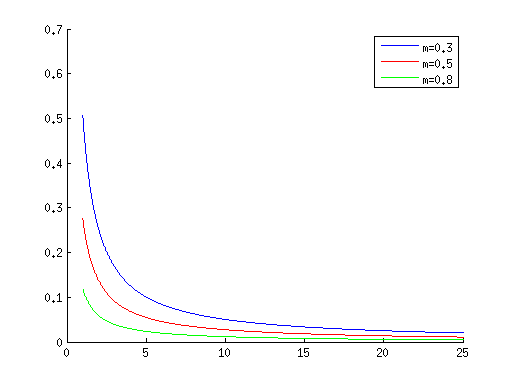
\includegraphics[scale=0.8]{R1C1.png}
\caption{Valeurs maximales de $\tau = R_1C_1$ en fonction de $F$, pour différentes valeurs de $m$}
\end{figure}

\item Lorsque $m \rightarrow 1$, $R_1C_1 \rightarrow 1$ : la modulation de la sinusoïde est trop importante pour pouvoir être suivie par le condensateur. Lorsque la fréquence du signal modulant se rapproche de la fréquence de la porteuse, on ne détecte plus rien car la détection suit les crêtes de la porteuse.
\end{itemize}

\newpage

\subsection{Démodulation cohérente}

\subsubsection{Principe de la démodulation cohérente et intérêt}

\begin{figure}[h!]
\centering
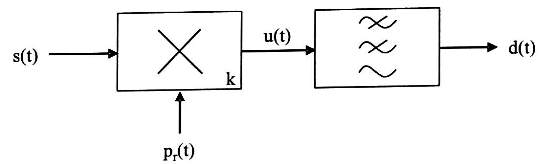
\includegraphics[scale=0.5]{detec.png}
\caption{Structure de principe d'un détecteur cohérent}
\end{figure}

On considère d'abord $p_r(t)$ identique à la porteuse $p(t)$.
Ainsi, on a 
\begin{multicols}{2}
DBPC :
\begin{align*}
u(t) & = kp(t)^2(1+ks_{inf}(t)) \\
& = \frac{kS_p^2}{2}(1+\cos(2\omega_0 t))(1+m\cos(\Omega t)) 
\end{align*}
Le spectre comporte des raies à $\Omega$, $2\omega_0$, $2\omega_0+\Omega$, $2\omega_0-\Omega$.

DBPS :
\begin{align*}
u(t) & = k^2p(t)^2s_{inf}(t)\\
& = \frac{k^2S_p^2}{2}\cos(\Omega t)(1+\cos(2\omega_0 t))
\end{align*}
Le spectre comporte des raies à $\Omega$, $2\omega_0+\Omega$, $2\omega_0-\Omega$
\end{multicols}

Comme $\Omega << \omega_0$, si on utilise un passe-bas qui laisse passer $\Omega$ mais coupe le reste, on restitue bien le signal modulant.\\


On considère maintenant $p_r(t)$ déphasée d'un angle $\phi$ par rapport à $p(t)$.

On a donc 
\begin{align*}
u(t) & = (1+s_{inf}(t))p(t)p_r(t) \\
& = (1+m\cos(\Omega t))S_p\cos(\omega_0 t)S_p\cos(\omega_0 t + \phi) \\
& = S_p^2(\frac{\cos(2\omega_0 t + \phi) + \cos(\phi)}{2}+\frac{m}{2}(\cos(\phi)\cos(\Omega t) + \frac{\cos((2\omega_0-\Omega)t+\phi) + \cos((2\omega_0+\Omega)t+\phi)}{2}))
\end{align*}

Après filtrage, il ne reste qu'une composante continue et une composante à $\Omega$ dont l'amplitude (positive par définition) varie en $|\cos(\phi)|$.

\subsubsection{Dimensionnement du filtre passe-bas}
On utilise un filtre passe-bas du second ordre réalisé par une structure de Rauch.
\[F_{PB}(p)=\frac{-1}{1+3R_0C_2p+R_0^2C_1C_2p^2}\]

\begin{figure}[h!]
\centering
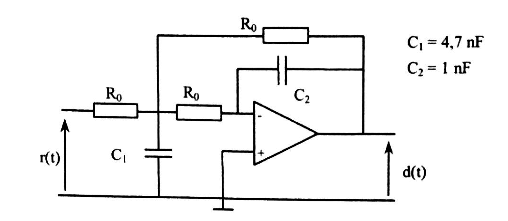
\includegraphics[scale=0.5]{PB.png}
\caption{Filtre passe-bas (Structure de Rauch)}
\end{figure}

On a donc $\omega_{0PB} = \frac{1}{R_0\sqrt{C_1C_2}}$ et $\xi=\frac{3}{2}\sqrt{\frac{C_2}{C_1}}$

On impose un coefficient d'amortissement du filtre $\xi=\frac{1}{\sqrt{2}}$, ce qui est bien vérifié avec les valeurs de $C_1$ et $C_2$.

Pour avoir une fréquence de coupure $f_c=20kHz$, il faut $R_0=3,7 k\Omega$.
\section{Étude d'une chaîne de transmission}

\subsection{Modélisation du canal de transmission}


\begin{figure}[h!]
\centering
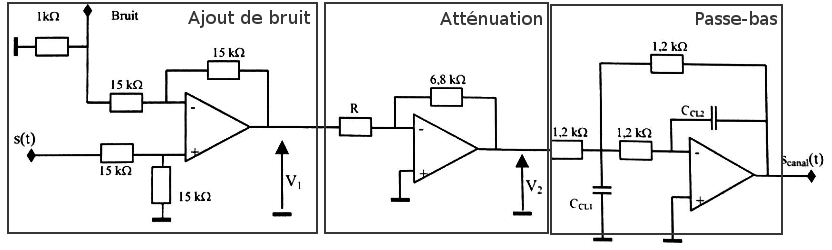
\includegraphics[scale=0.4]{canal.png}
\caption{Modélisation du canal de transmission}
\end{figure}


\begin{itemize}
\item \emph{Étude du bloc qui ajoute le bruit.} \\
Au bornes de l'amplificateur opérationnel
\begin{align*}
V_- & = \frac{B/R+V_1/R}{2/R} = \frac{B+V_1}{2} \\
V_+ & = \frac{S/R}{2/R} = \frac{S}{2}
\intertext{En considérant l'amplificateur parfait :}
V_1 & = \frac{S-B}{2}
\end{align*}

\item \emph{Fonction de transfert du filtre passe-bas utilisé}\\
\[F_{PB}(p)=\frac{-1}{1+3R_0C_{CL2}p+R_0^2C_{CL1}C_{CL2}p^2} \quad \avec R_0=1,2k\Omega \]

On a donc $\omega_{0PB} = \frac{1}{R_0\sqrt{C_{CL1}C_{CL2}}}$ et $\xi=\frac{3}{2}\sqrt{\frac{C_{CL2}}{C_{CL1}}}$.\\


On impose un coefficient d'amortissement du canal $\xi=\frac{1}{\sqrt{2}}$, donc $\frac{3}{2}\sqrt{\frac{C_{CL2}}{C_{CL1}}}=\frac{1}{\sqrt{2}}$ soit \[\frac{C_{CL2}}{C_{CL1}}=\frac{2}{9}\]

\item \emph{Atténuateur} : on a $\frac{V_2}{6,8k\Omega}+\frac{V_1}{R}=0$ donc l'atténuateur a un gain de $-\frac{R}{6,8k\Omega}$.
\end{itemize}

\newpage
\begin{center}
\begin{Large}
B. Expérimentation
\end{Large}
\end{center}

\setcounter{section}{0}

\section{Caractéristiques de la modulation d'amplitude}

Le multiplieur AD633 effectue l'opération
\[S = kXY + W\]

Dans un premier temps, on veut mettre $W$ à 0 donc on relie les bornes $B$ et $gnd$ avec un fil.

\begin{itemize}
\item On applique sur les deux entrées la même tension sinusoïdale, de fréquence 10kHz, d'amplitude 1V.

\begin{figure}[h!]
\centering
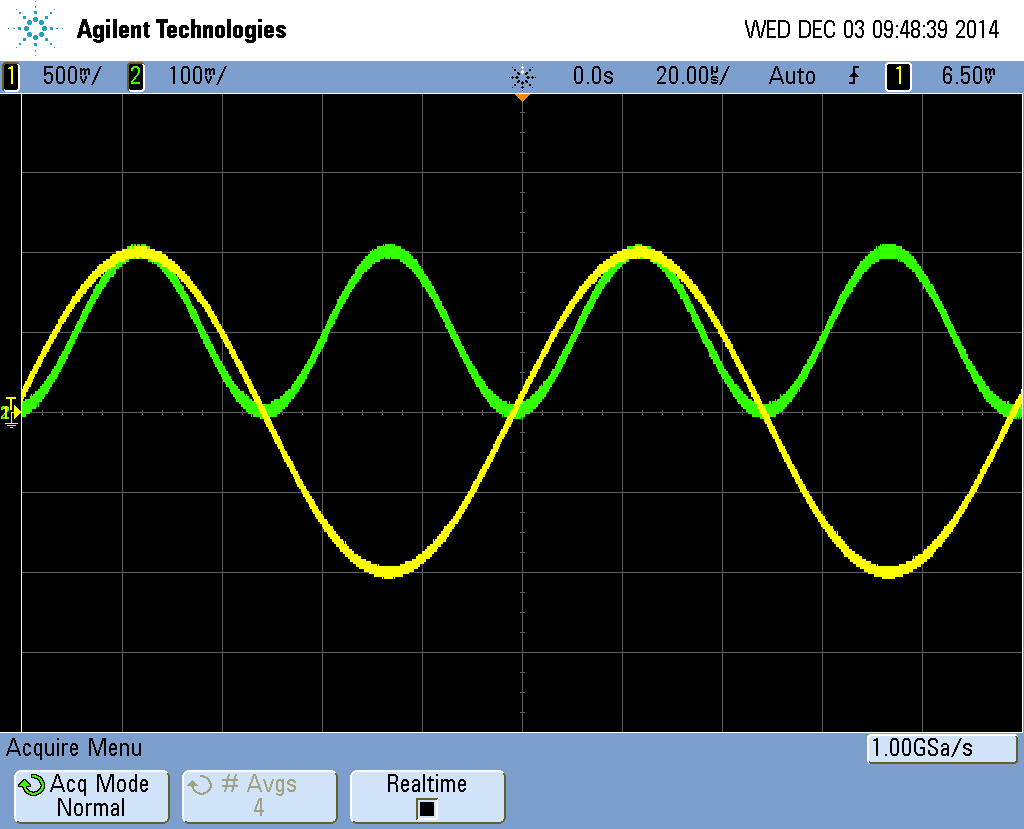
\includegraphics[scale=0.2]{gain_k.png}
\caption{$s(t)=kx_0^2\sin^2(\omega_0 t)$, $x_0=1V$, $f_0=10kHz$}
\end{figure}

On obtient un signal $s(t)=s_0\sin^2(\omega_0 t)$, avec $s_0=100mV$. On en déduit donc $k=0,1$.

La valeur de $k$ ne change pas à 70kHz.

\item On applique sur une des entrées le signal modulant de fréquence 5kHz et sur l'autre le signal porteur à 70kHz. Pour l'instant, on est en DBPS car on ne fait que multiplier les deux entrées entre elles

\begin{figure}[h!]
\centering
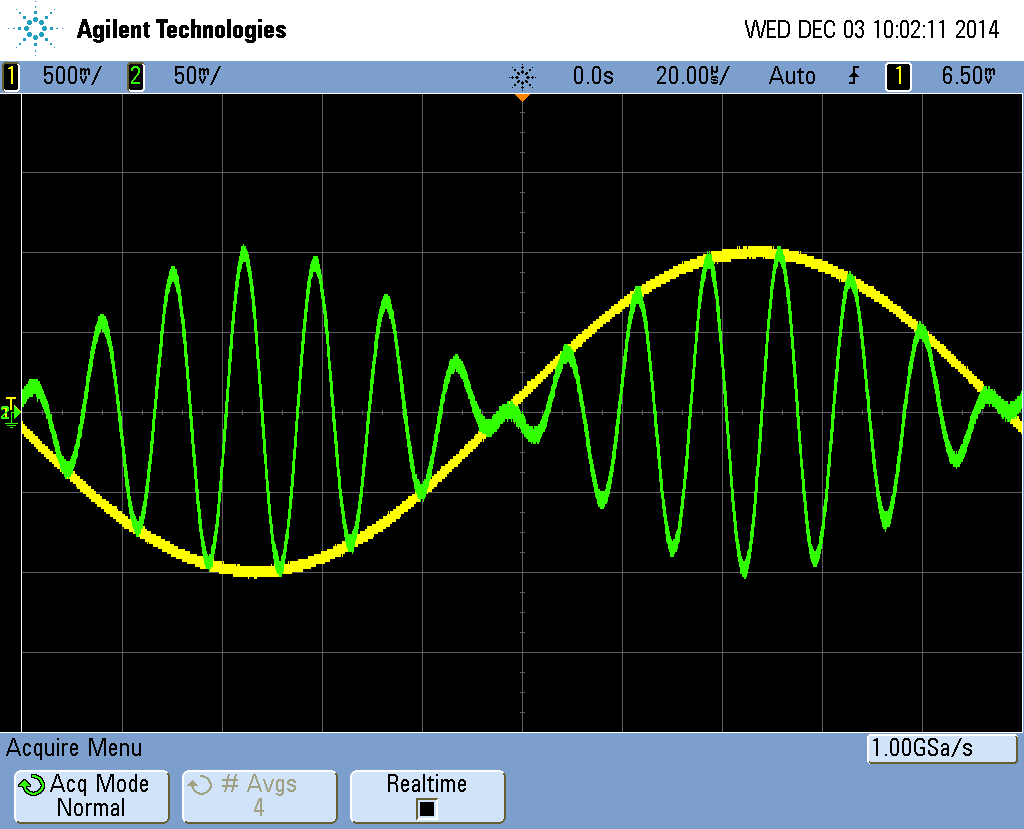
\includegraphics[scale=0.2]{DBPS705.png}
\caption{DBPS : $s(t)=kp(t)s_{inf}(t)$, modulante $F=5kHz$, porteuse $f_0=70kHz$}
\end{figure}

On observe bien une porteuse à 70kHz modulée par la modulante à 5kHz.
\end{itemize}



\subsection{Cas de la modulation D.B.P.C.}

Pour réaliser une DBPC, on relie les bornes A et B sur la plaquette à l'aide d'un filtre. Cela revient à ajouter la porteuse au signal de sortie :
\[s(t) = kS_pS_m[\cos(\omega_0 t)\cos(\Omega t)]+S_p\cos(\omega_0 t)\]

\subsubsection*{Modulation classique}
\begin{figure}[h!]
\centering
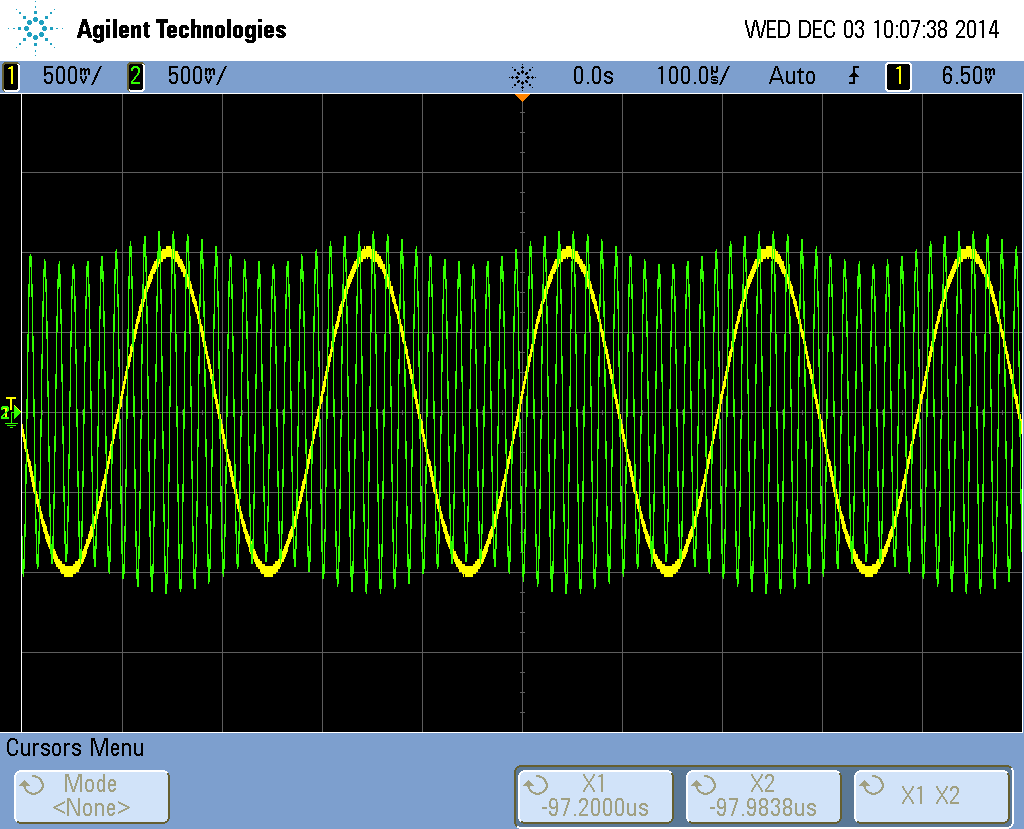
\includegraphics[scale=0.2]{DBPC1.png}
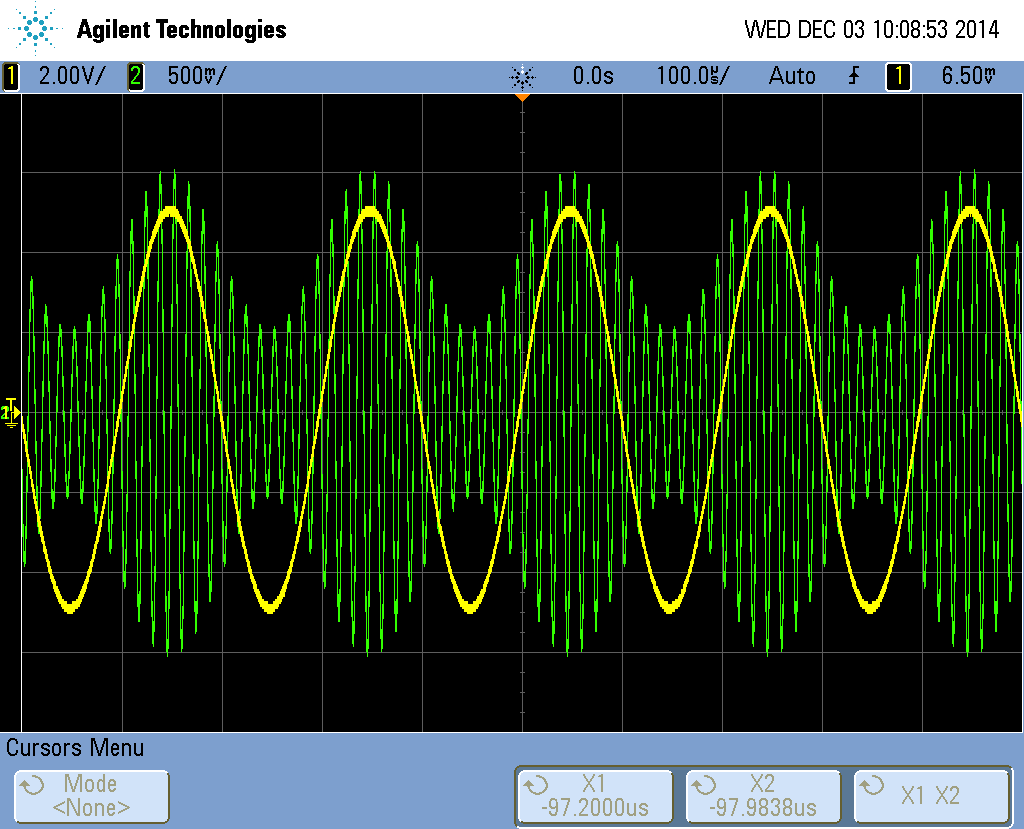
\includegraphics[scale=0.2]{DBPC5.png}
\caption{Signal temporel $s(t)$ en modulation classique, avec $S_m=1V$ puis $S_m=5V$}
\end{figure}

Pour le second cas, on voit que l'amplitude de la modulation est de 4V, et la valeur moyenne de 4V. D'après la préparation, en notant $Max$ le maximum de l'enveloppe du signal, $min$ le minimum, on a
\[m= 2\frac{Max-min}{Max+min}\] donc on a ici $m=0,5$. Ceci correspond à la valeur attendue, car avec $S_m=5V$, $m=kS_m=0,5$.

\begin{figure}[h!]
\centering
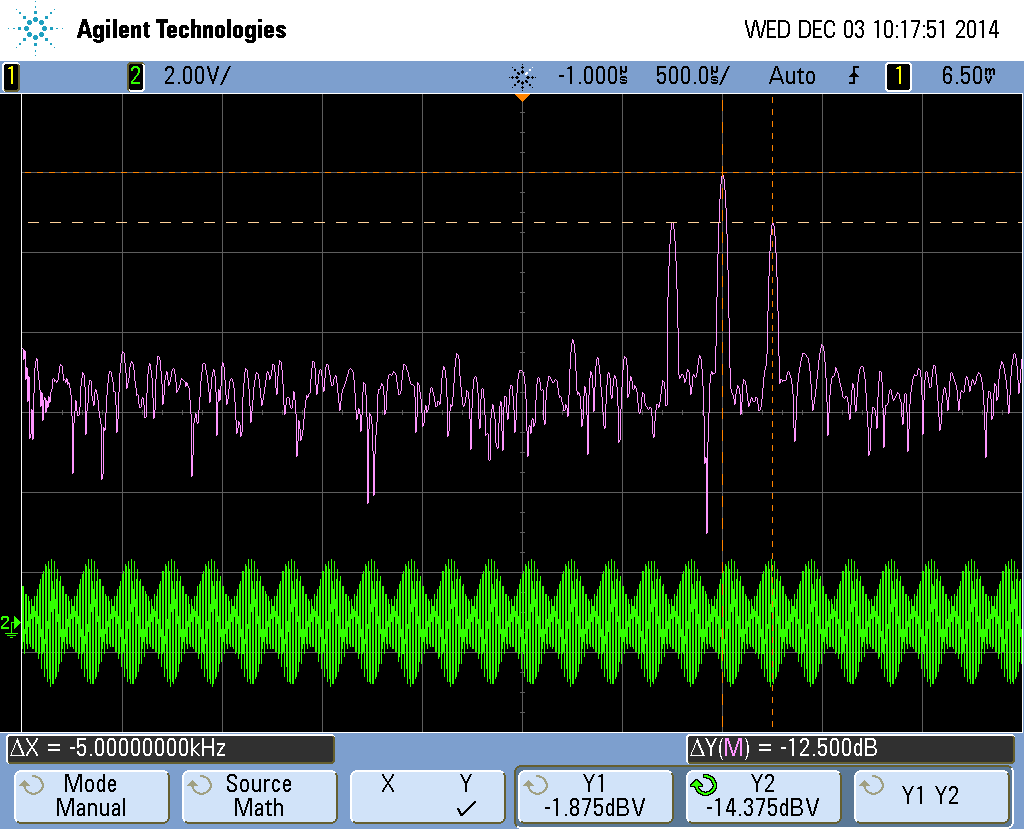
\includegraphics[scale=0.2]{DBPC5FFT.png}
\caption{FFT de $s(t)$ en modulation classique, FFT, avec $S_m=5V$}
\end{figure}

D'après la préparation , si on note $A_{\omega_0}$ (resp. $A_{\omega_0-\Omega}$) l'amplitude de la composante à $\omega_0$ (resp. $\omega_0-\Omega$) de $s(t)$, alors \[m=\frac{2A_{\omega_0-\Omega}}{A_{\omega_0}}\]

Ainsi, avec $\Delta(Y)$ le rapport en dB des amplitudes des pics déterminés par FFT sur l'oscilloscope, \[m=2*10^{\frac{\Delta(Y)}{20}}\]

On mesure $\Delta(Y)=-12.5dB$. On peut donc en déduire $m=0.47$.\\

On retrouve donc bien par les deux méthodes (visualisation temporelle et analyse spectrale) la valeur du taux de modulation attendue.

\subsubsection*{Surmodulation}
\begin{figure}[h!]
\centering
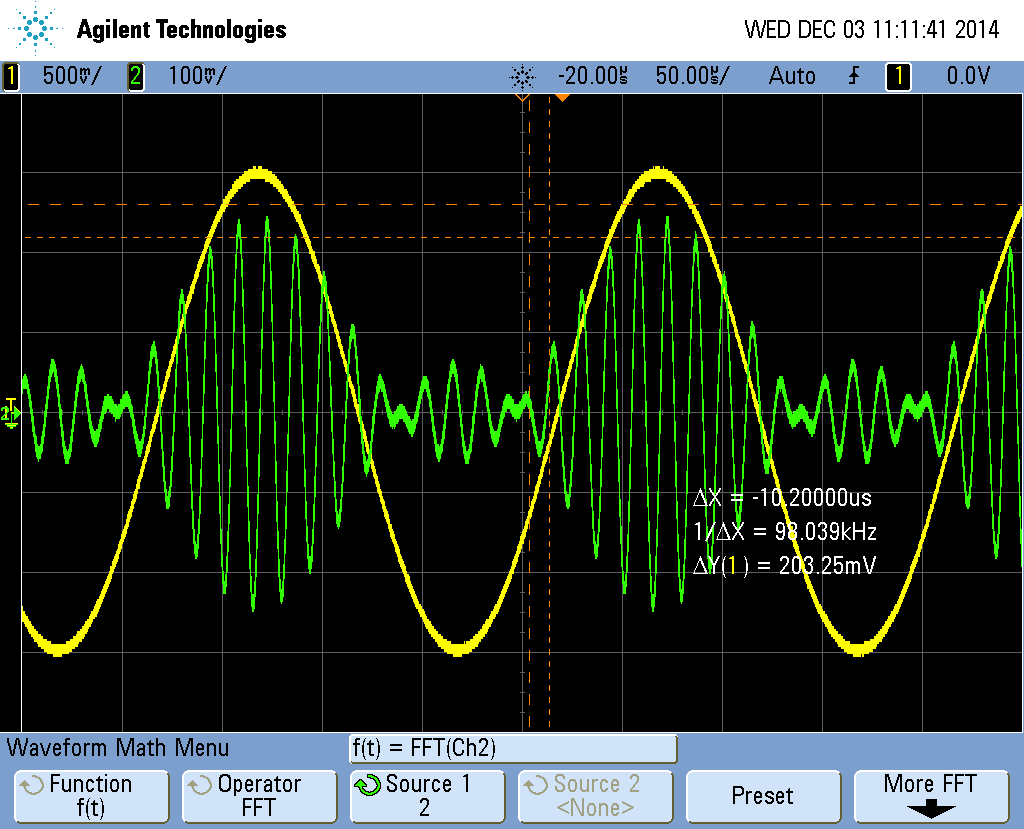
\includegraphics[scale=0.2]{Surmod.png}
\caption{Signal temporel $s(t)$ en surmodulation, avec $S_m=1,5V$ et pont diviseur de gain 0,1}
\end{figure}

On réalise à l'aide d'un pont diviseur :
\[s(t) = kS_pS_m[\cos(\omega_0 t)\cos(\Omega t)]+0,1S_p\cos(\omega_0 t)\]

On a donc le taux de modulation $m=\frac{kS_pS_m}{0,1S_p}=1,5$ avec $S_p=1V$.

On peut le retrouver expérimentalement : l'amplitude de la modulation est de 0,75V, et sa valeur moyenne est 0,5V.

On a donc \[m= 2\frac{Max-min}{Max+min}=0,75/0,5 = 1,5\]

\newpage
\subsection{Cas de la modulation D.B.P.S}

Le signal modulé est alors :
\[s(t)=kS_pS_m[\cos(\Omega t)\cos(\omega_0 t)]\]

\begin{figure}[h!]
\centering
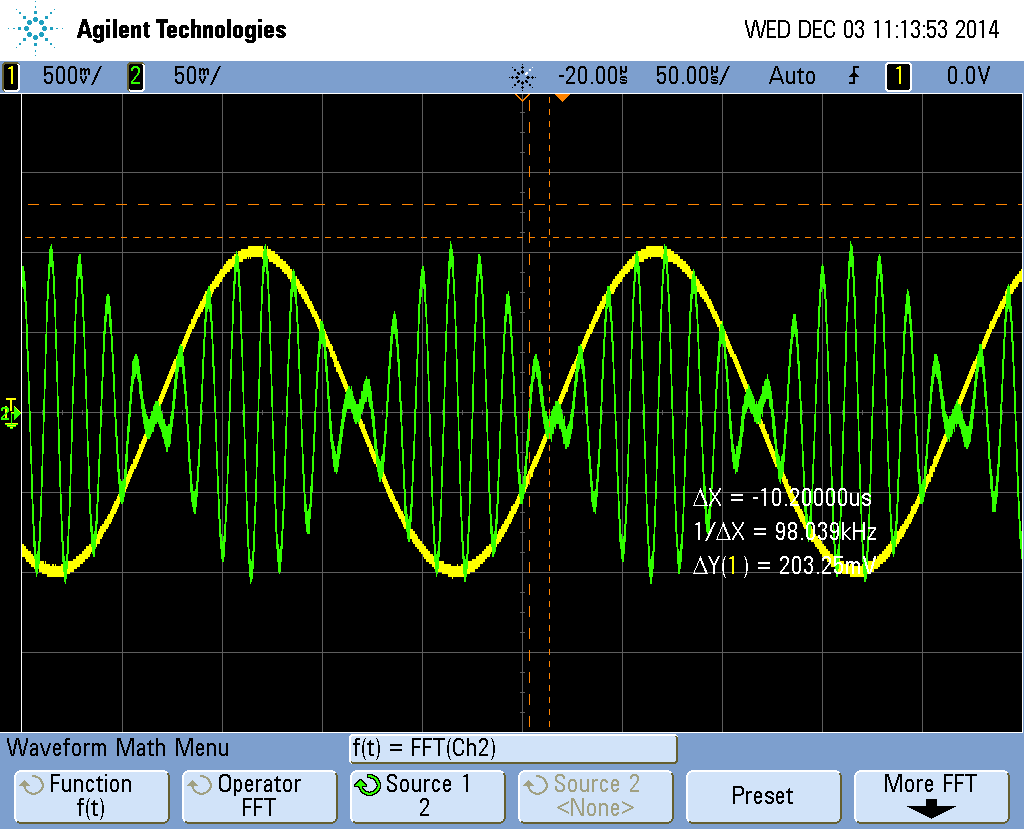
\includegraphics[scale=0.2]{DBPS1.png}
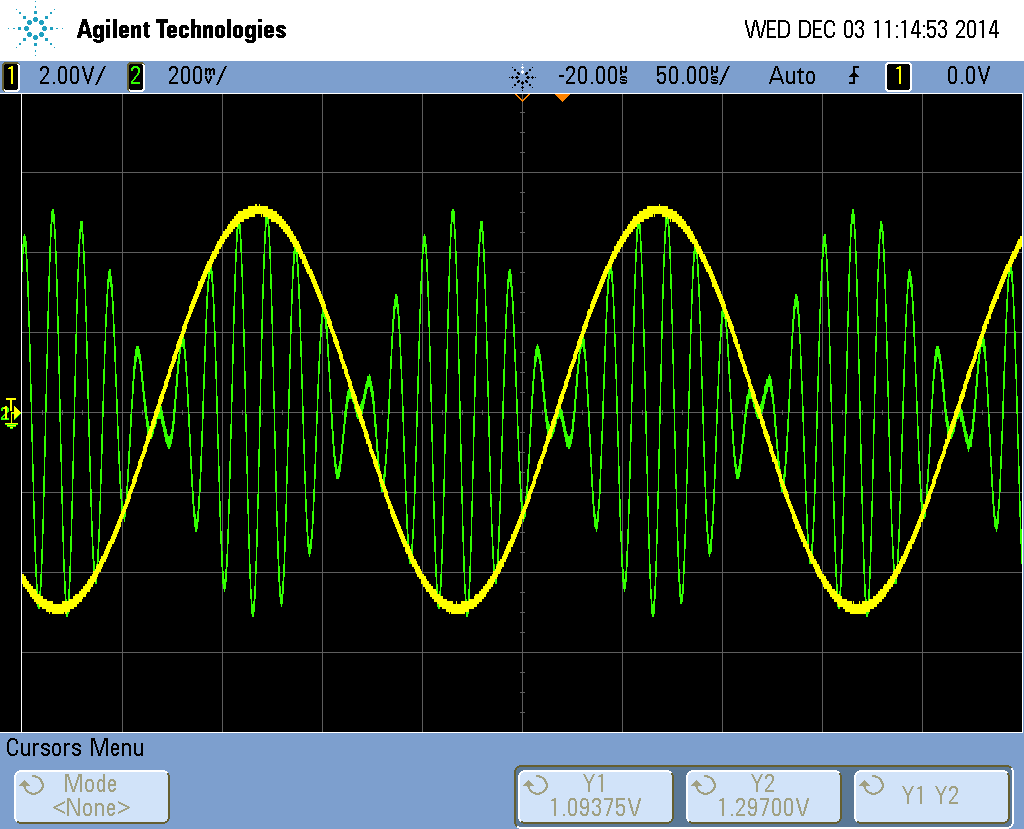
\includegraphics[scale=0.2]{DBPS5.png}
\caption{Signal temporel $s(t)$, avec $S_m=1V$ puis 5V}
\end{figure}

\begin{figure}[h!]
\centering
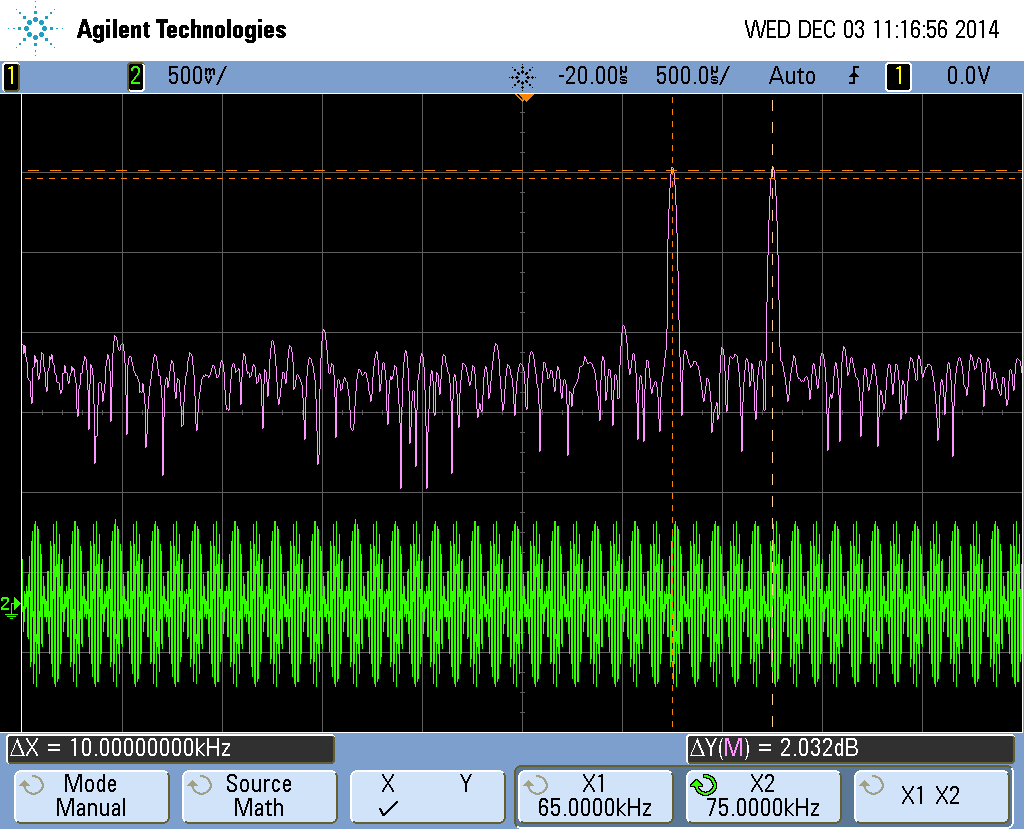
\includegraphics[scale=0.2]{DBPS5FFT.png}
\caption{FFT de $s(t)$, avec $S_m=1V$}
\end{figure}

\newpage
\section{Techniques de démodulation d'amplitude}

\subsection{Démodulation par détection d'enveloppe}

On réalise un détecteur d'enveloppe avec $R_1=15k\Omega$ et $C_1=15nF$.\\

Dans un premier temps, on regarde l'influence de $m$.
\begin{figure}[h!]
\centering
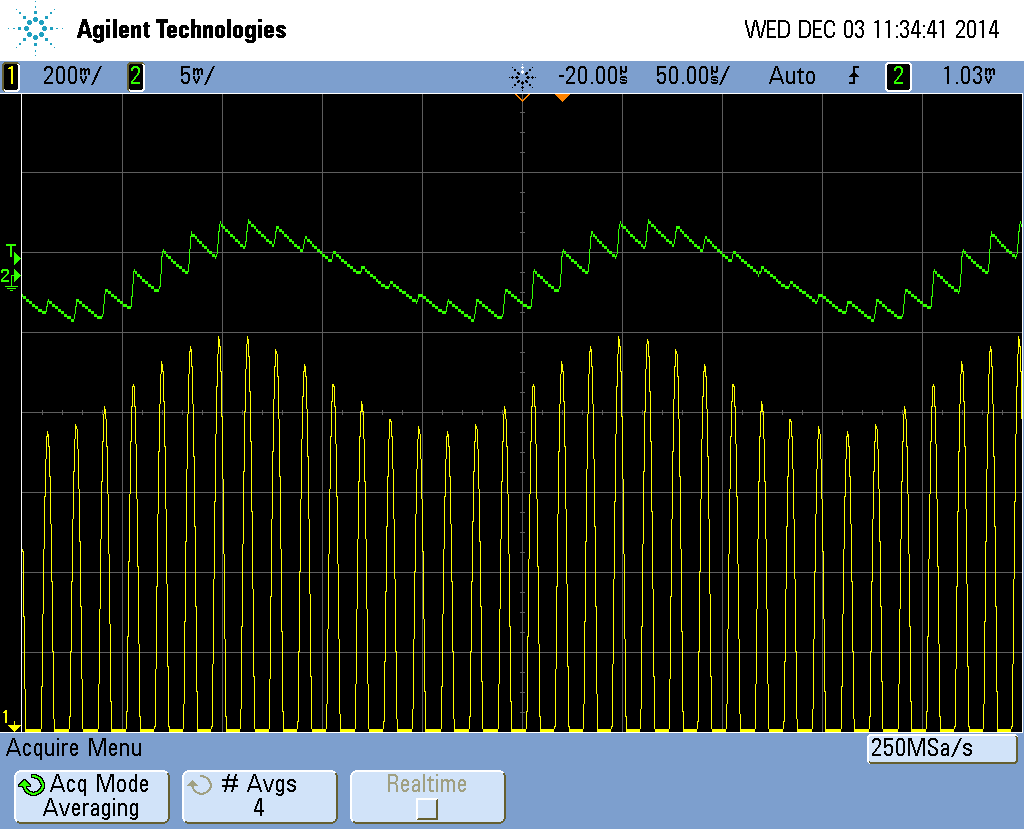
\includegraphics[scale=0.2]{DEOK.png}
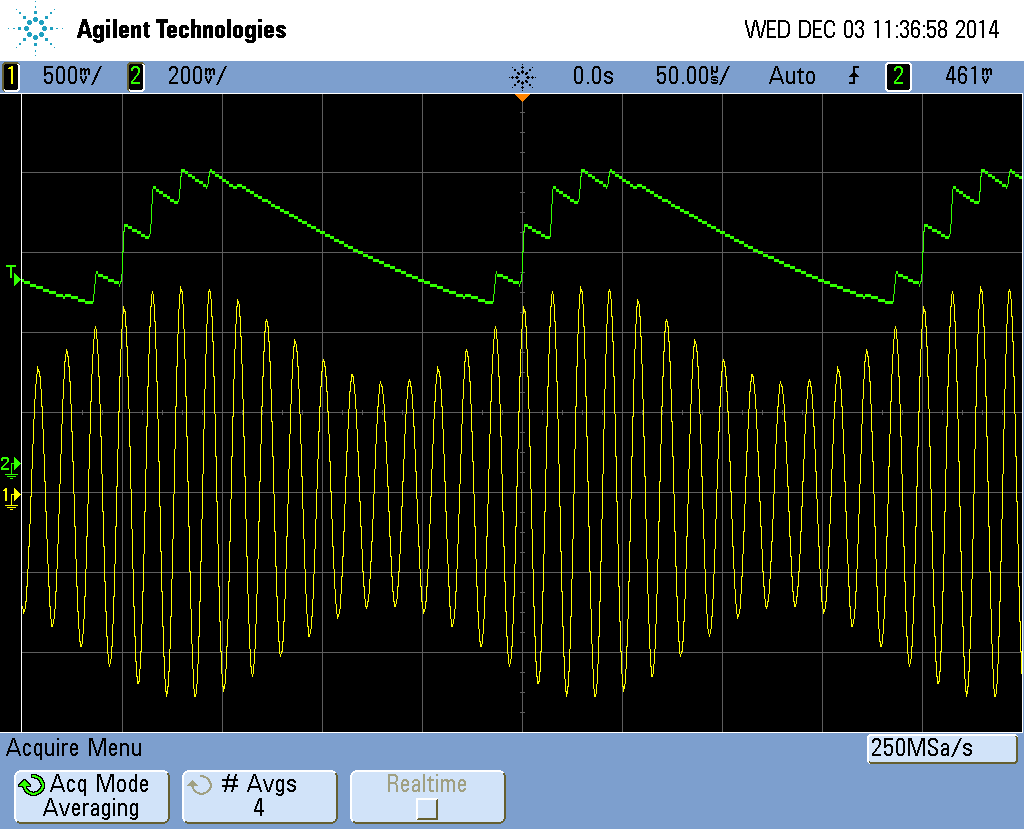
\includegraphics[scale=0.2]{DEKO.png}
\caption{Détection d'enveloppe, $F=5kHz$, $m=0,1$ puis 0,4}
\end{figure}

On remarque que lorsque $m$ s'approche de 1, la détection se détériore. C'est ce qui avait été prévu en préparation : la décharge du condensateur est trop lente (par rapport aux variations de la modulante) pour suivre la modulation.

\begin{figure}[h!]
\centering
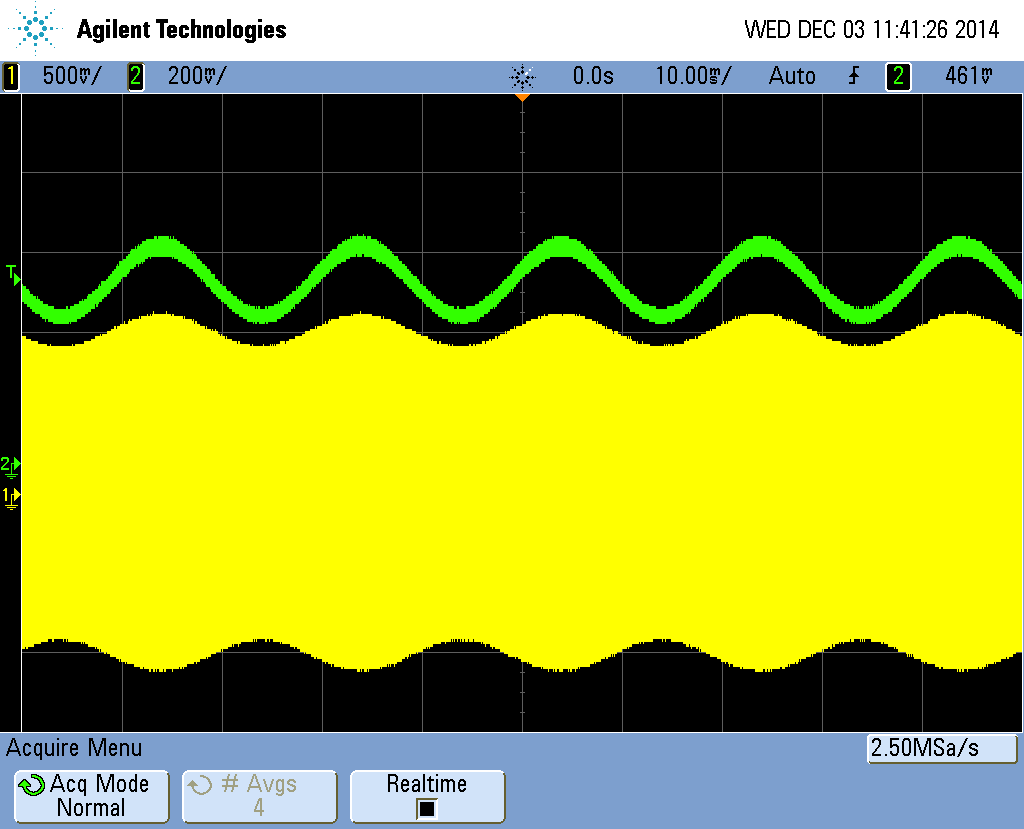
\includegraphics[scale=0.2]{DEBF.png}
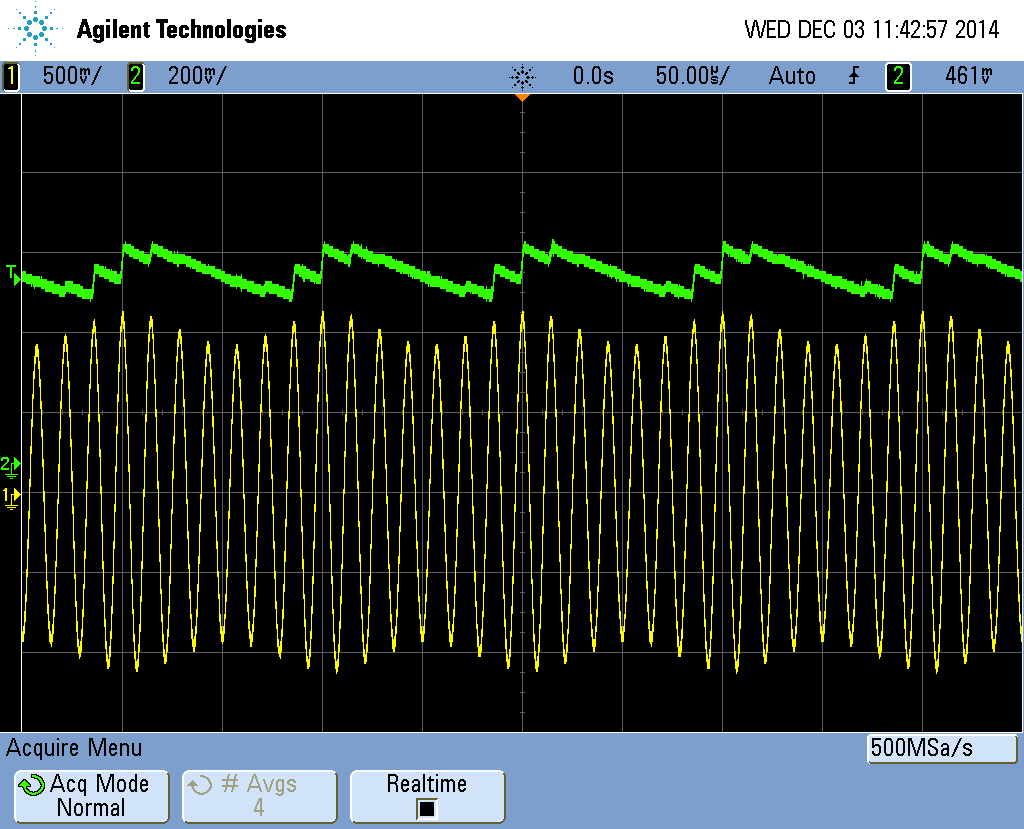
\includegraphics[scale=0.2]{DEHF.png}
\caption{Détection d'enveloppe, $F=50Hz$ puis $10kHz$, $m=0,1$}
\end{figure}

À basse fréquence, le signal modulant est bien restitué. À haute fréquence, la décharge du condensateur est trop lente (par rapport à la fréquence de la modulante) pour suivre la modulation.

\begin{figure}[h!]
\centering
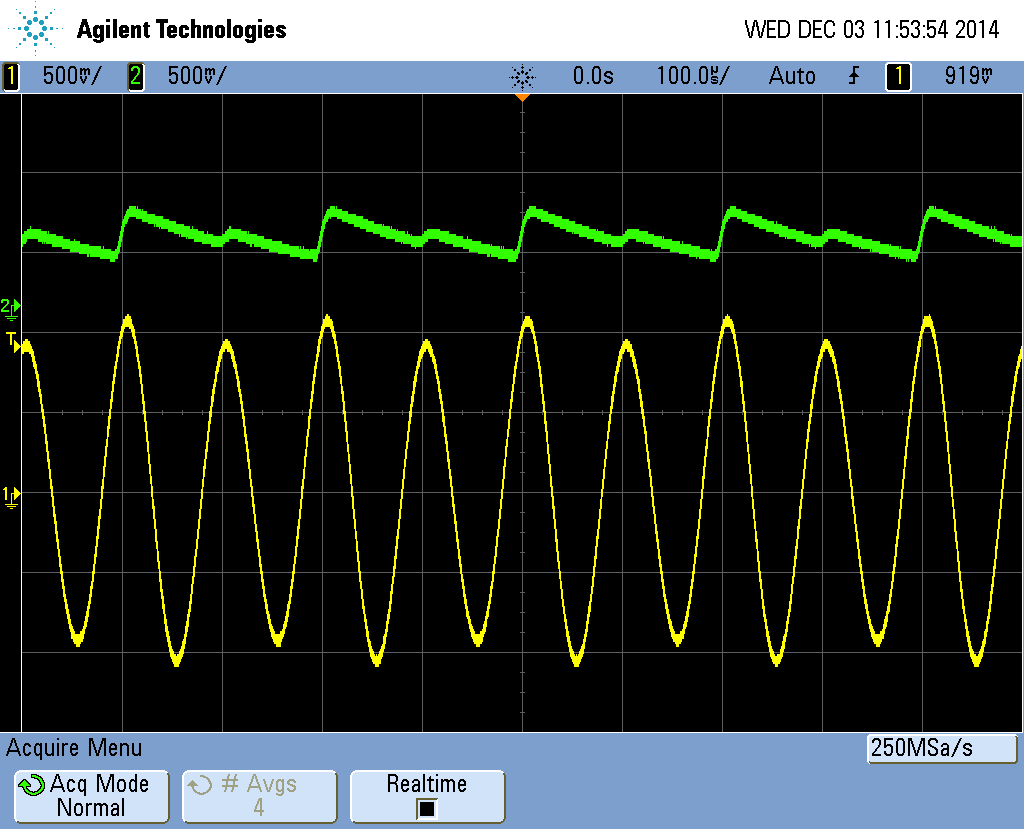
\includegraphics[scale=0.2]{DE2F.png}
\caption{Détection d'enveloppe pour $f_0=2F$}
\end{figure}

Lorsque la fréquence de la porteuse est proche de $2F$, la détection ne peut plus se faire car les fréquences sont trop proches pour pouvoir voir la modulation. 

\newpage
\subsection{Démodulation par détection synchrone : démodulation cohérente}

On utilise le GBF 2 voies pour générer la porteuse et un signal synchrone avec la porteuse, avec un déphasage variable.\\

Le signal en entrée du filtre est :
\[u(t)  = (1+s_{inf}(t))p(t)p_r(t)  = (1+m\cos(\Omega t))S_p\cos(\omega_0 t)S_p\cos(\omega_0 t + \phi) \]
On filtre et on ne récupère que la composante représentant la modulante . On relève son amplitude en fonction du déphasage entre porteuse et porteuse reconstituée.

\begin{figure}[h!]
\centering
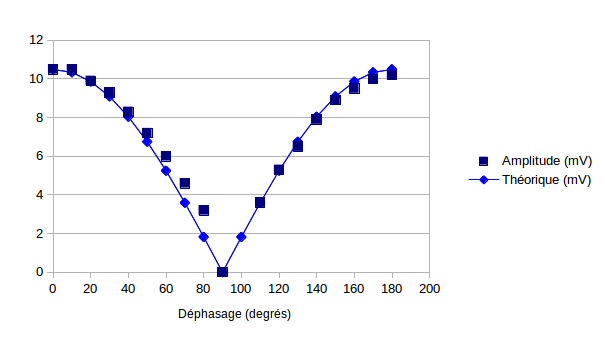
\includegraphics[scale=0.8]{Graphe.png}
\caption{Amplitude du signal démodulé en fonction du déphasage entre $p(t)$ et $p_r(t)$}
\end{figure}

On retrouve une loi correspondant à un cosinus (en valeur absolue). 

On montre donc qu'il est important d'avoir une porteuse et une porteuse reconstituée en phase pour récupérer le maximum de signal en sortie. Cependant, la démodulation synchrone fonctionne si le déphasage entre les deux signaux $p(t)$ et $p_r(t)$ reste faible.

\newpage
\section{Étude de la démodulation d'un signal bruité}

\subsection{Le canal de transmission}

On trace le diagramme de Bode du canal de transmission. Celui-ci devait avoir une fréquence de coupure de l'ordre de 100kHz et un amortissement proche de 0,707. \\
Avec $R=6,8k\Omega$, pour avoir les conditions $\frac{C_{CL2}}{C_{CL1}}=0,22$ et $C_{CL1}C_{CL2}=5,5.10^{-20}$, on prend pour valeur numérique des condensateurs $C_1 = 330 pF$ et $C_2 = 100 pF$.

\begin{figure}[h!]
\centering
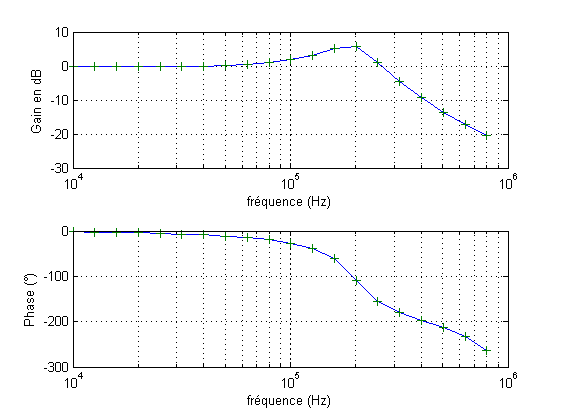
\includegraphics[scale=0.7]{BodeCacanal.png}
\caption{Diagramme de Bode du canal de transmission}
\end{figure}

Le filtre est bien un passe-bas d'ordre 2 de fréquence de coupure autour de $100kHz$.

\subsection{Influence du bruit vis-à-vis de la démodulation synchrone}

On introduit volontairement du bruit dans la transmission et on observe le signal de sortie. Pour un bruit modéré, le signal modulé est encore reconnaissable :

\begin{figure}[h!]
\centering
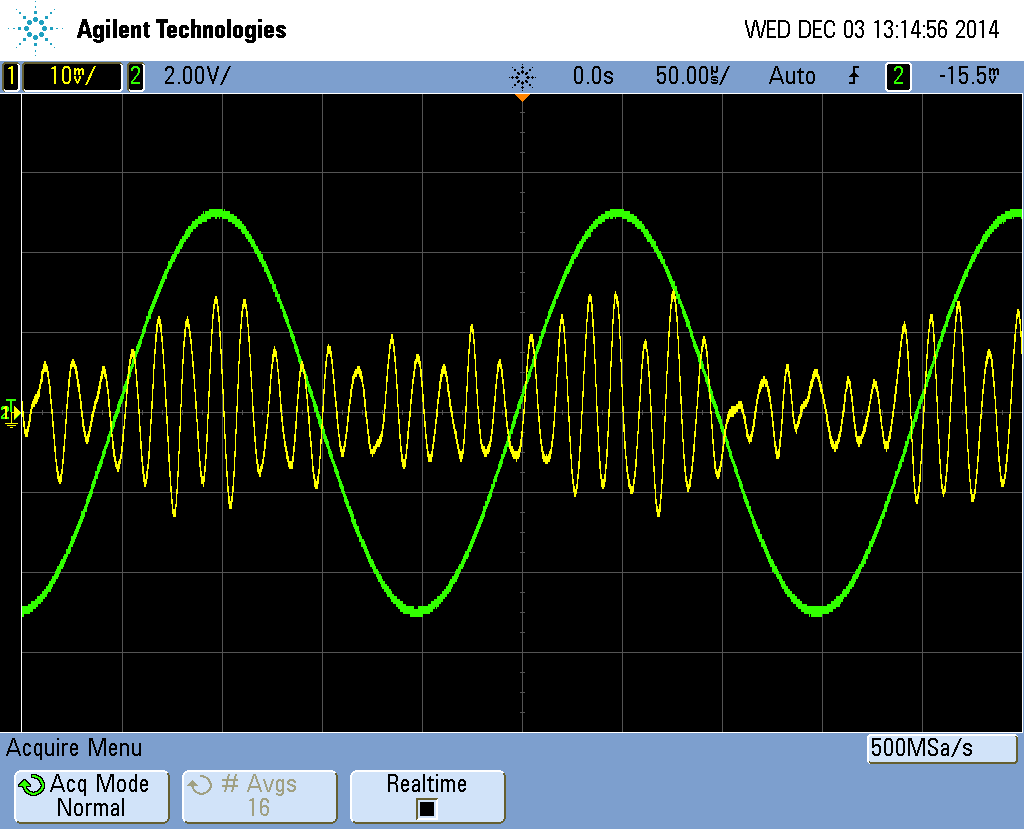
\includegraphics[scale=0.2]{NoiseMod.png}
\caption{Signaux modulant et modulé, bruit modéré}
\end{figure}

Lorsque le signal est fortement bruité, (ici, l'amplitude du bruit est égale à l'amplitude de la modulante) le signal reconstitué est lui aussi fortement bruité mais la détection est tout de même réalisée :

\begin{figure}[h!]
\centering
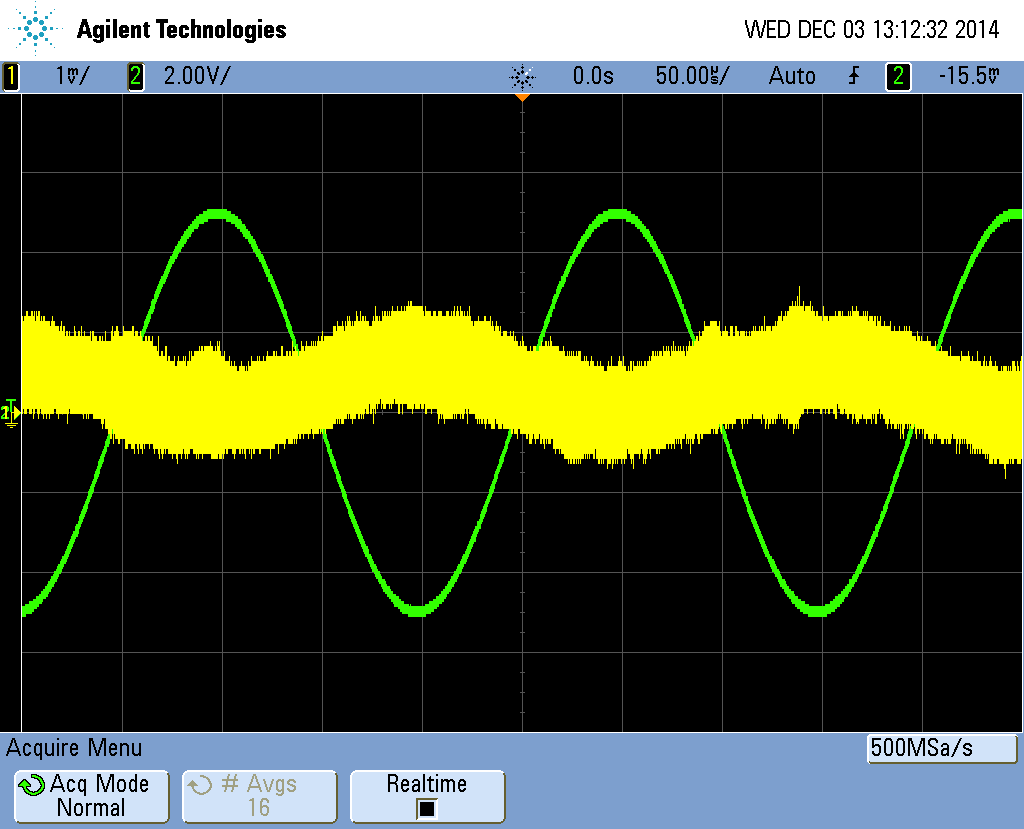
\includegraphics[scale=0.2]{NoiseMAX.png}
\caption{Signaux modulant et démodulé, bruit fort}
\end{figure}

Si le bruit reste limité, on montre que la démodulation est d'assez bonne qualité. En effet, on peut tracer la FFT du signal modulé en sortie du canal de transmission :

\begin{figure}[h!]
\centering
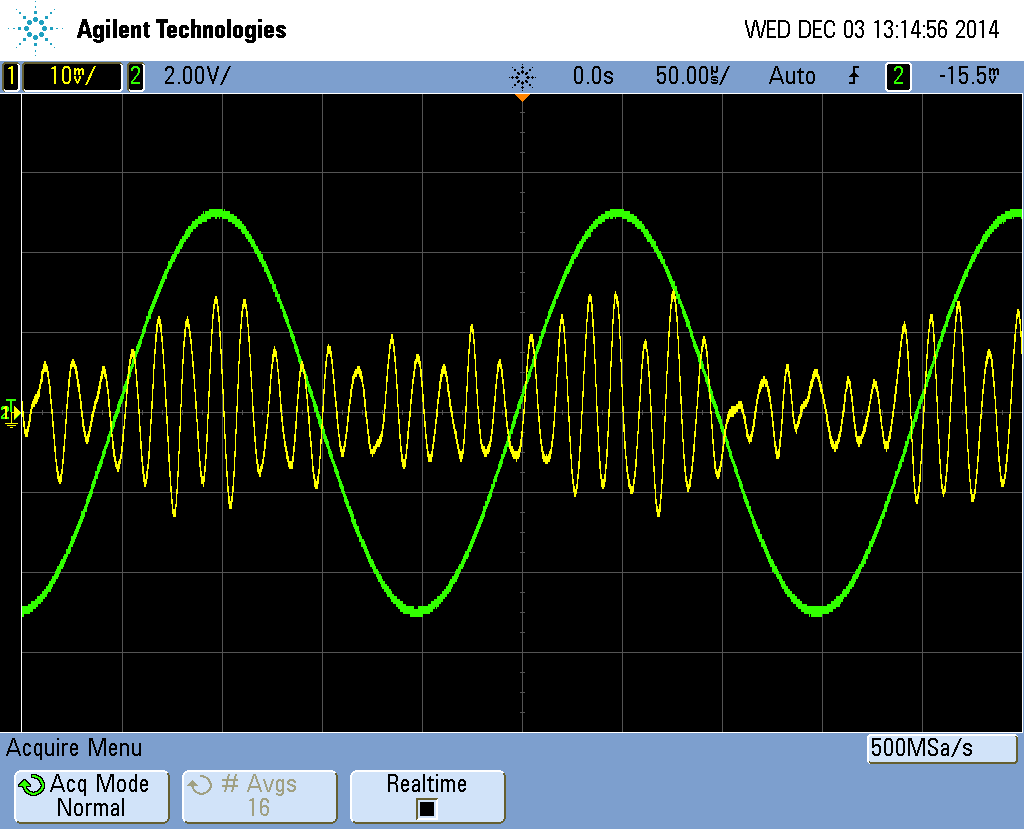
\includegraphics[scale=0.2]{NoiseMod.png}
\caption{Signal modulé transmis (en haut), signal démodulé (au milieu) et sa FFT (en bas)}
\end{figure}

Le signal démodulé est une sinusoïde bruité. Sa FFT présente un pic à 5kHz, ce qui montre qu'on récupère effectivement une modulante altérée.\\

La détection synchrone permet, même en cas de signal fortement bruité, de récupérer de façon acceptable le signal modulant.
\end{document}
